\documentclass[a4paper]{article}

\usepackage[T1]{fontenc}
\usepackage[utf8]{inputenc}
\usepackage[french]{babel}
\usepackage{mathpazo}
\usepackage[scaled]{helvet}
\usepackage{courier}
\usepackage[sf,bf]{titlesec}
\usepackage[margin=0.75in]{geometry}
\usepackage{tabularx}
\usepackage{graphicx}
\usepackage{caption}

\setlength{\parindent}{4em}
\setlength{\parskip}{1em}

\makeatletter
\newenvironment{expl}{%
  \begin{list}{}{%
    \small\itshape%
    \topsep\z@%
    \listparindent0pt%\parindent%
    \parsep0.75\baselineskip%\parskip%
    \setlength{\leftmargin}{20mm}%
    \setlength{\rightmargin}{20mm}%
  }
    \item[]}%
    {\end{list}}
\makeatother

% Indiquez votre prénom (en minuscules) et votre nom (en majuscules)
\title{Rapport de TP \\ Architecture des systèmes d'exploitation}
\author{\underline{Paul} \underline{MEYER}}
\date{Novembre 2021}

\begin{document}

  \maketitle

% Mettez une table des matières si votre rapport contient plus
% de 3 pages ou si vous ne suivez pas le plan suggéré :
  \tableofcontents

  \listoffigures

% Dans votre rapport final, supprimez toutes les explications
% (c'est-à-dire tous les environnements \begin{expl} ... \end{expl}).
  \newpage

  \section{Introduction}

  L'objectif de ce TP est d'implémenter un vaccinodrome qui prend en charge des patients, venant se faire vacciner par des médecins. Les médecins vaccinent les patients dans des box, ces derniers attendront donc à l'extérieur jusqu'à
  ce qu'il y ait une place dans la salle d'attente. Une fois dans la salle d'attente le patient attendra sur un siège numéroté qu'un médecin soit disponible. Lorsqu'un médecin sera disponible, le patient entrera dans le box pour se faire vacciner, puis partira une fois l'action réalisée. Les médecins attendrons jusqu'à la fermeture du vaccinodrome pour partir.

  Dans cette implémentation, nous avons laisser le patient choisir un box disponible.
  Lorsqu'un médecin est disponible, le patient en sera informé et cherchera le box disponible.
  Une fois le box monopolisé, le patient notifiera le médecin qu'il veut être vacciné et restera dans le box pour toute la durée de la vaccination, en attendant que le médecin le laisse partir. En partant, le box sera libéré et un nouvelle notification de disponibilité du médecin sera envoyée aux patients.
  \newpage
  \section{Structure de données}

  \subsection{Structures de données partagées}\label{sec-shm}

  J'ai utilisé un total de 3 structures, toutes font partie de la mémoire partagée.

  La structure principale s'appelle vaccinodrome\_t et contient toutes les données utiles, sémaphores, et variables globales.

  \begin{tabularx}{\linewidth}{|l|l|l|X|}
    \hline
    % \multicolumn{4}{|l|}{Distributeur de gel
    %   (\texttt{struct distr\_gelha})}
    % \\ \hline
    Champ & Type & Init & Description \\ \hline%
    nbSieges & int & -- & Nombre de sièges dans le vaccinodrome. \\ \hline%
    nbMedecins & int & -- & Nombre de médecins dans le vaccinodrome. \\ \hline%
    temps & int & -- & Temps pris par une vaccination en ms. \\ \hline%

    waitingRoom & asem\_t & nbSieges & Sémaphore qui gère l'accès a la salle d'attente. \\ \hline%
    medecinDisponibles & asem\_t & 0 & Sémaphore qui notifie lorsqu'un médecin est disponible. \\ \hline%
    fermer & asem\_t & 0 & Sémaphore qui attends la fermeture de tous les médecins. \\ \hline%

    asemMutex & asem\_t & 1 & Sémaphore binaire qui sert de "mutex" lors d'un accès a la mémoire partagée box\_t. \\ \hline%
    siegeMutex & asem\_t & 1 & Sémaphore binaire qui sert de "mutex" lors d'un accès a la mémoire partagée siege\_t. \\ \hline%
    waitingMutex & asem\_t & 1 & Sémaphore binaire qui sert de "mutex" lors d'un accès a la variable currPatientWaiting. \\ \hline%

    currMedecins & int & 0 & Nombre médecins actuellement dans le vaccinodrome. \\ \hline%
    currPatientWaiting & int & 0 & Nombre de patients attendant à l'extérieur du vaccinodrome. \\ \hline%
    statut & int & 0 & Statut de fermeture/ouverture du vaccinodrome (0 ouvert, 1 fermé) \\ \hline%
    medecins & box\_t[] & -- & Flexible array contenant les boxes de médecins \\ \hline%

  \end{tabularx}
  \\[12pt]
  La seconde structure s'appelle box\_t, et contient toutes les informations d'un box.

  \begin{tabularx}{\linewidth}{|l|l|l|X|}
    \hline
    % \multicolumn{4}{|l|}{Distributeur de gel
    %   (\texttt{struct distr\_gelha})}
    % \\ \hline
    Champ & Type & Init & Description \\ \hline%
    demandeVaccin & asem\_t & 0 & Sémaphore qui attends qu'un patient demande un vaccin au médecin. \\ \hline%
    termineVaccin & asem\_t & 0 & Sémaphore notifiant le patient lorsqu'il a été vacciné. \\ \hline%
    status & int & 0 & Statut du box (0 libre, 1 occupé, 2 fermé) \\ \hline%
    medecin & int & -- & Nombre de médecins dans le vaccinodrome. \\ \hline%
    patient & char[] & -- & Nom du patient pris en charge \\ \hline%

  \end{tabularx}
  \\[12pt]
  La troisième structure s'appelle siege\_t, et contient toutes les informations d'un siège.

  \begin{tabularx}{\linewidth}{|l|l|l|X|}
    \hline
    % \multicolumn{4}{|l|}{Distributeur de gel
    %   (\texttt{struct distr\_gelha})}
    % \\ \hline
    Champ & Type & Init & Description \\ \hline%
    siege & int & -- & Id (numéro) du siège \\ \hline%
    statut & int & 0 & Statut du siège (0 libre, 1 occupé) \\ \hline%

  \end{tabularx}

  \subsection{Structures de données non partagées}

  \begin{expl}
    Aucune donnée utile n'est pas partagée.
  \end{expl}

  \newpage

  \section{Synchronisations}

  \subsection{Arrivée d'un patient}\label{arrivee-patient}

  Lorsqu'un patient arrive, on vérifie directement si le vaccinodrome est ouvert. Si ce n'est pas le cas, on arrête le programme. Ensuite, on attend qu'une place dans la salle d'attente se libère et lorsqu'une place est libre on vérifie à nouveau si le vaccinodrome est ouvert (et on arrête le programme si ça ne passe pas). Sachant qu'une place s'est libérée, on cherche le siège disponible et on l'affecte au patient.
  Finalement, on attend qu'un box (médecin) soit libre.

  \begin{enumerate}
    \item Les objets impliqués sont :

    \begin{tabularx}{\linewidth}{|l|l|>{\strut}X|}
      \hline%
      waitingRoom & asem\_t & Sémaphore qui gère l'accès a la salle d'attente \underline{du vaccinodrome}. \\ \hline%
      currPatientWaiting & int & Nombre de patients attendant à l'extérieur \underline{du vaccinodrome} \\ \hline%
      medecinDisponibles & asem\_t & Sémaphore qui notifie lorsqu'un médecin est disponible. \\ \hline%
      siegeMutex & asem\_t & Sémaphore binaire qui sert de "mutex" lors d'un accès a la mémoire partagée siege\_t. (\underline{vaccinodrome}) \\ \hline%
      waitingMutex & asem\_t & Sémaphore binaire qui sert de "mutex" lors d'un accès a la variable currPatientWaiting. (\underline{vaccinodrome}) \\ \hline%
      statut & int & Statut de fermeture/ouverture du vaccinodrome (0 ouvert, 1 fermé) \\ \hline%
    \end{tabularx}

    \item Pour l'arrivée d'un patient seul, on exécute le programme "patient".

    \begin{verbatim}
// Ce code est exécuté par le patient

// On veut vérifier si le vaccinodrome n'est pas fermé
verifier_statut_vaccinodrome(statut)

// On souhaite avoir le nombre exact de patients qui
// attendent devant la porte
P (waitingMutex)
currPatientWaiting++;
V (waitingMutex)

// On attend qu'une place se libère dans la salle d'attente
P (waitingRoom)

// Le patient est rentré, on peut décrémenter
P (waitingMutex)
currPatientWaiting--;
V (waitingMutex)

// On veut à nouveau vérifier si le vaccinodrome n'est pas fermé
verifier_statut_vaccinodrome(statut)

// On cherche le siège disponible où le patient attendra
P (siegeMutex)
chercher_siege()
V (siegeMutex)

// On attends qu'un médecin soit disponible
P (medecinDisponibles)

    \end{verbatim}

    \item L'implémentation du nombre de clients devant la porte me sert de repère quand je lance fermer,
    afin de débloquer le nombre exact de patients derrière la porte pour qu'ils puissent partir, et pour afficher un debug lors du test 200. La sémaphore waitingRoom est initialisée à N sièges, donc elle gère automatiquement le nombre de patients dans la salle d'attente.
  \end{enumerate}
  \newpage
  \subsection{Arrivée d'un médecin}

  Lorsqu'un médecin arrive, on vérifie directement si le vaccinodrome est ouvert. Si ce n'est pas le cas, on arrête le programme. Puis on vérifie s'il n'y a pas déjà trop de médecins (si oui, on arrête le programme). On incrémente le nombre de médecins actuels, puis on initialise le box.
  Finalement on notifie les patients que le médecin est disponible et on attend une demande de vaccination.

  \begin{enumerate}
    \item Les objets impliqués sont :

    \begin{tabularx}{\linewidth}{|l|l|>{\strut}X|}
      \hline%
      asemMutex & asem\_t & Sémaphore binaire qui sert de "mutex" lors d'un accès a la mémoire partagée box\_t. (\underline{vaccinodrome}) \\ \hline%
      medecinDisponibles & asem\_t & Sémaphore qui notifie lorsqu'un médecin est disponible. \\ \hline%

      nbMedecins & int & Nombre de médecins dans le \underline{vaccinodrome}. \\ \hline%
      currMedecins & int & Nombre médecins actuellement dans le \underline{vaccinodrome}. \\ \hline%
      statut & int & Statut de fermeture/ouverture du \underline{vaccinodrome} (0 ouvert, 1 fermé) \\ \hline%

      demandeVaccin & asem\_t & Sémaphore qui attends qu'un patient demande un vaccin au médecin. (\underline{box}) \\ \hline%
      termineVaccin & asem\_t & Sémaphore notifiant le patient lorsqu'il a été vacciné. (\underline{box}) \\ \hline%
      status & int & Statut du \underline{box} (0 libre, 1 occupé, 2 fermé) \\ \hline%
    \end{tabularx}

    \item Pour l'arrivée d'un médecin, seul est exécuté le programme "médecin".

    \begin{verbatim}
// Ce code est exécuté par le médecin

// On veut vérifier si le vaccinodrome n'est pas fermé
verifier_statut_vaccinodrome(statut)

// On veut vérifier qu'il n'y a pas trop de médecins
verifier_place_medecin(currMedecins, nbMedecins)

// Un médecin en plus !
P (asemMutex)
currMedecins++;

// On initialise le box ainsi que ses sémaphores
init_box()
asem_init(demandeVaccin, termineVaccin)
box->status = 0

V (asemMutex)

// On notifie les patients qu'un médecin est disponible
V (medecinDisponibles)

// On démarre la boucle qui traite les demandes de vaccins
While :
    P(demandeVaccin)
    // On attend qu'un patient entre dans le box et demande la vaccination

    \end{verbatim}

    \item Sachant que le patient s'occupe de trouver un box disponible, il faut impérativement bloquer l'accès à la liste des boxes avant que le box soit bien initialisé, (sinon il pourrait y avoir des accès concurrents à ce box non initialisé).
  \end{enumerate}
  \newpage

  \subsection{Interactions entre patients et médecins}


  Lorsqu'un médecin est disponible, le patient va chercher et s'attribuer un box disponible. Il va quitter son siège et notifier aux autres patients qu'une place dans la salle d'attente s'est libérée. Puis il va demander au médecin de le vacciner, et attendre jusqu'à ce qu'il le relâche. Le médecin va donc se réveiller et vérifier la raison de son réveil (s'il doit s'arrêter ou parce qu'un patient la révéillé). Puis il va vacciner le patient, et le relâcher. Finalement, il remet son box en disponibilité et notifie tous les patients qu'il est à nouveau disponible, avant d'attendre la prochaine demande de vaccination.

  \begin{enumerate}
    \item Les objets impliqués sont :

    \begin{tabularx}{\linewidth}{|l|l|>{\strut}X|}
      \hline%
      asemMutex & asem\_t & Sémaphore binaire qui sert de "mutex" lors d'un accès a la mémoire partagée box\_t. (\underline{vaccinodrome}) \\ \hline%
      medecinDisponibles & asem\_t & Sémaphore qui notifie lorsqu'un médecin est disponible. (\underline{vaccinodrome}) \\ \hline%
      waitingRoom & asem\_t & Sémaphore qui gère l'accès a la salle d'attente. (\underline{vaccinodrome}) \\ \hline%
      nbMedecins & int & Nombre de médecins dans le \underline{vaccinodrome}. \\ \hline%
      currMedecins & int & Nombre médecins actuellement dans le \underline{vaccinodrome}. \\ \hline%
      statut & int & Statut de fermeture/ouverture du \underline{vaccinodrome} (0 ouvert, 1 fermé) \\ \hline%
      temps & int & Temps pris par une vaccination en ms (\underline{vaccinodrome}). \\ \hline%

      demandeVaccin & asem\_t & Sémaphore qui attends qu'un patient demande un vaccin au médecin. (\underline{box}) \\ \hline%
      termineVaccin & asem\_t & Sémaphore notifiant le patient lorsqu'il a été vacciné. (\underline{box}) \\ \hline%
      status & int & Statut du \underline{box} (0 libre, 1 occupé, 2 fermé) \\ \hline%
      patient & char[] & Nom du patient pris en charge (\underline{box})\\ \hline%
      statut & int & Statut du \underline{siège} (0 libre, 1 occupé) \\ \hline%
    \end{tabularx}

    \item Les programmes exécutés sont "medecin" et "patient".

    \begin{verbatim}
// Ce code est exécuté par le patient

// On attend un médecin disponible
P (medecinDisponibles)

// On cherche un box et on le réserve pour le patient
P (asemMutex)
chercher_box()
box->status = 1
box->patient = patient
V (asemMutex)

// On rend le siege a nouveau disponible
P (siegeMutex)
siege->statut = 0
V (siegeMutex)

// On notifie les autres patients qu'une place s'est libérée
// dans la salle d'attente
V (waitingRoom)

// On notifie le medecin que l'on souhaite être vacciné
V (demandeVaccin)

// Puis on attend que le médecin nous relâche
P (termineVaccin)

// Le patient est vacciné
    \end{verbatim}
    \newpage

    \begin{verbatim}
// Ce code est exécuté par le médecin

// On attend qu'un patient entre dans le box et demande la vaccination
P(demandeVaccin)

// On vérifie la raison du réveil
P (siegeMutex)
verifier_fermeture()
V (siegeMutex)

// La vaccination dure un certain temps...
usleep(temps)

// On laisse partir le patient
V (termineVaccin)

// On remet le statut du box à 0.
P (asemMutex)
liberer_box()
V (asemMutex)

// On vérifie s'il y a encore un patient à vacciner ou non
P (siegeMutex)
verifier_fermeture()
V (siegeMutex)

// Le médecin est à nouveau disponible
V (medecinDisponibles)

// On redémarre la boucle... attente d'un patient à vacciner...

    \end{verbatim}

    \item Il faut faire attention aux variables critiques, l'accès aux sièges ainsi qu'aux box est ouverte. Si deux patients souhaitent accéder au même box il pourrait y avoir une erreur. C'est pour cela que j'utilise ici deux sémaphore binaires en guise de mutex.
  \end{enumerate}
  \newpage

  \subsection{Fermeture du vaccinodrome}

  Lors de la fermeture, on change le statut du vaccinodrome à "fermé".
  Puis, s'il y a plus aucun patient dans la salle d'attente, on notifie les médecins qui sont disponible de se fermer. S'il y'a encore des sièges occupés, on laisse partir des potentiels patient qui attendraient devant la salle (s'il y'en a). Puis on attend la fermeture de tous les médecins avant de quitter le programme.


  \begin{enumerate}
    \item Les objets impliqués sont :

    \begin{tabularx}{\linewidth}{|l|l|>{\strut}X|}
      \hline%
      asemMutex & asem\_t & Sémaphore binaire qui sert de "mutex" lors d'un accès a la mémoire partagée box\_t. (\underline{vaccinodrome}) \\ \hline%
      waitingRoom & asem\_t & Sémaphore qui gère l'accès a la salle d'attente. (\underline{vaccinodrome}) \\ \hline%
      fermer & asem\_t & Sémaphore qui attends la fermeture de tous les médecins du \underline{vaccinodrome}. \\ \hline%
      currMedecins & int & Nombre médecins actuellement dans le \underline{vaccinodrome}. \\ \hline%
      statut & int & Statut de fermeture/ouverture du \underline{vaccinodrome} (0 ouvert, 1 fermé) \\ \hline%

      demandeVaccin & asem\_t & Sémaphore qui attends qu'un patient demande un vaccin au médecin. (\underline{box}) \\ \hline%
      status & int & Statut du \underline{box} (0 libre, 1 occupé, 2 fermé) \\ \hline%
      statut & int & Statut du \underline{siège} (0 libre, 1 occupé) \\ \hline%
    \end{tabularx}

    \item Le programme exécuté est "fermer"

    \begin{verbatim}
// Ce code est exécuté par fermer

// Le vaccinodrome est dès à présent fermé
statut = 1

// On veut récuperer le nb de sièges occupés dans la salle d'attente
P (siegeMutex)
count_sieges_occupes()
V (siegeMutex)

Si sieges_occupes = 0:
    Pour tous les médecins actuels:
        P (asemMutex)
        Si médecin disponible:
            status = 2 // Le statut est changé à fermé

            // on débloque le médecin qui vérifiera la raison de son réveil.
            V (demandeVaccin)
        V (asemMutex)
Sinon:
    Pour tous les patients qui attendent à l'extérieur:
        V (waitingRoom) // On débloque les patients afin qu'ils s'arrêtent

// On attend que tous les médecins se terminent
Pour tous les médecins actuels:
    P (fermer)

    \end{verbatim}

    \item Lors de la fermeture il faut bien vérifier à ne pas réveiller des médecins qui sont déjà entrain de vacciner des patients. De plus, il faut aussi veiller à ne pas changer le statut d'un box en même temps qu'un patient au risque de se retrouver avec un problème de concurrence.
  \end{enumerate}
  \newpage

  \subsection{Patients après fermeture}

  Seuls les patients qui tentent de rentrer dans la salle d'attente seront automatiquement rejetés.
  Sinon un patient étant dans la salle d'attente avant la fermeture, aura un déroulement normal.

  \begin{enumerate}
    \item Les objets impliqués sont :

    \begin{tabularx}{\linewidth}{|l|l|>{\strut}X|}
      \hline%
      waitingRoom & asem\_t & Sémaphore qui gère l'accès a la salle d'attente. (\underline{vaccinodrome}) \\ \hline%

      waitingMutex & asem\_t & Sémaphore binaire qui sert de "mutex" lors d'un accès a la variable currPatientWaiting. (\underline{vaccinodrome}) \\ \hline%
      currPatientWaiting & int & Nombre de patients attendant à l'extérieur \underline{du vaccinodrome} \\ \hline%
      statut & int & Statut de fermeture/ouverture du \underline{vaccinodrome} (0 ouvert, 1 fermé) \\ \hline%
    \end{tabularx}

    \item Le programme exécuté est "patient"

    \begin{verbatim}
// Ce code est exécuté par le patient (copié de la partie 3.1)

...

// On attend qu'une place se libère dans la salle d'attente
P (waitingRoom)

// Le patient est rentré, on peut décrémenter
P (waitingMutex)
currPatientWaiting--;
V (waitingMutex)

// On vérifie donc ici si le vaccinodrome est fermé,
// si c'est le cas on rejette ce patient et on termine le programme.
verifier_statut_vaccinodrome(statut)
    \end{verbatim}

    \item Aucun problème par ici.
  \end{enumerate}
  \newpage

  \subsection{Médecins après fermeture}

  Lors de la fermeture, les médecins qui ne sont pas entrain de vacciner sont réveillés avec la raison "fermeture". Ils vérifient qu'il n'y ait plus de patients dans la salle d'attente et se finissent.
  S'ils sont déjà entrain de vacciner une personne, et que le vaccinodrome est fermé, ils vérifient à nouveau à la fin de la vaccination si un patient est présent dans la salle d'attente. Si ce n'est pas le cas le médecin s'arrêtera.

  \begin{enumerate}
    \item Les objets impliqués sont :

    \begin{tabularx}{\linewidth}{|l|l|>{\strut}X|}
      \hline%
      asemMutex & asem\_t & Sémaphore binaire qui sert de "mutex" lors d'un accès a la mémoire partagée box\_t. (\underline{vaccinodrome}) \\ \hline%
      siegeMutex & asem\_t & Sémaphore binaire qui sert de "mutex" lors d'un accès a la mémoire partagée siege\_t. (\underline{vaccinodrome}) \\ \hline%
      fermer & asem\_t & Sémaphore qui attends la fermeture de tous les médecins du \underline{vaccinodrome}. \\ \hline%
      statut & int & Statut du \underline{siège} (0 libre, 1 occupé) \\ \hline%
      demandeVaccin & asem\_t & Sémaphore qui attends qu'un patient demande un vaccin au médecin. (\underline{box}) \\ \hline%
    \end{tabularx}

    \item Le programme exécuté est "medecin"

    \begin{verbatim}
// Ce code est exécuté par medecin

// On attend une demande de vaccin ou une fermeture
P (demandeVaccin)

// On vérifie si la raison du réveil est bien une fermeture
P (siegeMutex)

Si box->status == "terminé" et statut = "fermé" et sieges_occupes() == 0:
    Alors: Le medecin peut partir

V (siegeMutex)

...

// Lorsqu'un patient a été vacciné et que le vaccinodrome est fermé,
// on vérifie s'il y'a plus personne dans la salle d'attente.
// Si c'est le cas, alors le médecin peut partir
P (siegeMutex)

Si statut = "fermé" et sieges_occupes() == 0:
    Alors: Le medecin peut partir

V (siegeMutex)

...

// Avant de terminer chaque médecin change son statut à "fermé"
P (asemMutex)
box->status = "fermé"
V (asemMutex)

// et notifie sa fermeture via la sémaphore "fermer"
V (fermer)
    \end{verbatim}

    \item (Copie du 3.4) Lors de la fermeture il faut bien vérifier à ne pas réveiller des médecins qui sont déjà entrain de vacciner des patients. De plus, il faut aussi veiller à ne pas changer le statut d'un box en même temps qu'un patient au risque de se retrouver avec un problème de concurrence.
  \end{enumerate}
  \newpage

  \section{Remarques sur l'implémentation}

  Au niveau de la mémoire partagée j'ai fait le choix d'avoir deux tableaux, mais mettre un pointeur dans une structure n'était pas si simple que ça, donc j'ai fait le choix de mettre un flexible array dans la structure et de faire un pointeur externe, sans préciser de variable. Ce qui m'a donné les fonctions get\_sieges() et get\_siege\_at(index), dans la quelle on se positionne derrière l'adresse du flexible array.

  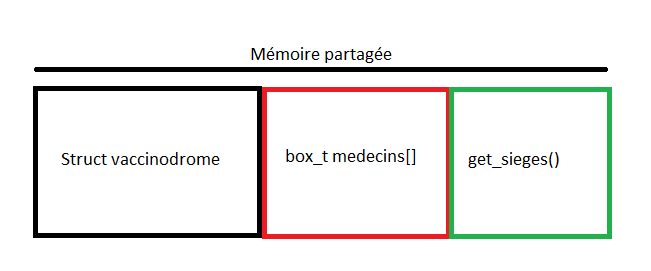
\includegraphics[scale=0.8]{mempartagee.png}
  \captionof{figure}{Schéma de la mémoire partagée}
  \label{fig1}

  De plus, j'aurais sûrement dû ajouter une section critique au niveau de la variable statut du vaccinodrome.

  \section{Conclusion}

  Grâce à ce projet j'ai réussi à mieux comprendre les sémaphores et sections critiques, c'était un super  entraînement à la synchronisation.\par
  Je ne vois pas particulièrement de limites à mon implémentation, à part de mémoire/CPU peut-être, car les programmes se démarrent/terminent indépendamment. Ceci dit, peut-être que s'il y a trop de sémaphores qui se bloquent/débloquent en même temps le CPU pourrait avoir des problèmes à gérer tout ça. Mais ce serait seulement dans le cas où il y aurait trop de programmes lancés en même temps.\par
  Ce choix d'implémentation impose quand même peu de liberté au médecin, c'est le patient qui gère tout, entrée dans le vaccinodrome, choix du siège, choix du box...\par
  J'ai eu des difficultés avec la mémoire partagée. Le tableau flexible dans la mémoire partagée fonctionnait, mais y ajouter un deuxième tableau m'a amené beaucoup de problèmes, car le pointeur n'était pas bien placé. Finalement j'ai réussi en utilisant l'arithmétique des pointeurs.

\end{document}